\section{Evaluation}\label{sec:eval}

We implemented the formal transformation rule for the distributed training
as a software. We designed the software to be a standalone software, so 
the ML developers can utilize the software regardless of their environment. 
The software is written in Scala; the source code and released software
is available at https://github.com/kaist-plrg/python-analyzer.

To evaluate the automated transformation tool, we set up two research
questions.

\begin{itemize}
\item RQ1. (Correctness) Does the tool correctly transform single-GPU based DL model codes into
the corresponding distributed model codes?

\item RQ2. (Effectiveness) Does the automatic transformation result in speed-up 
in distributed training compared to single-GPU training?
\end{itemize}

To answer these questions,  
we designed two experiments: \textbf{transformation experiment} and
\textbf{distributed training experiment}.
The transformation experiment aims to answer the RQ1; it tests if the
transformation tool correctly transforms the target model codes into
the answer code.
The distributed training experiment aims to answer the RQ2;
it measures the training speed of single-GPU based model and its
corresponding transformed distributed model and compare them.
In this section, we describe the experiment setting,
and discuss the results of the experiments and its implications.

\pagebreak
\subsection{Experiment Targets and Settings}

We gathered open-source TensorFlow DL model codes as the experiment target.
The full list of the experiment target models is described in the
figure \ref{fig:eval:targets}.
At first, we targetd the example model codes in the Horovod 
Github\cite{horovodgithub}. Although the Horovod GitHub repository provides
examples for various ML frameworks, we could only use two models based on the
TensorFlow frameworks. As a result, we searched for other GitHub repositories
that contain TensorFlow ML model codes.
The TensorFlow model garden\cite{tfmodelgarden} is one of the official
collections of ML models from TensorFlow.
Other sources\cite{tfexamplesdamien}\cite{cifar10github}\cite{tf2tutogithub} are
non-official ML examples that include various ML architectures.
We selected targets with various ML architectures to show that
our transformation tool works well regardless of the architecture types.

After gathering the models, we selected valid experiment targets to be used. 
We excluded some models from experiments to keep only trainable model codes. 
For example, the CycleGAN model in the TensorFlow 2.x tutorials
was unsuable because the training dataset was not accessible from the
Internet. Additionally we modified some parts of the model in order to patch
minor bugs in the code in training.
Then, we manually rewrite each model code into distributed model codes using
the Horovod library. The manually rewritten codes will be used as "answers" 
for the transform experiment.
For the case of Horovod GitHub example codes, which are distirbuted model
codes from the start, we manually inspect the codes and eliminate
Horovod library-related codes to rewrite them into single-GPU based
models, and use them as the target codes.

\begin{figure}[!ht]
  \begin{center}
  \begin{tabular}{c|c|l}
    \hline
    Model Name & API Pattern & Source \\
    \hline
    LSTM-MNIST & GradientTape & \multirow{2}{*}{TensorFlow Examples by Americ Damien\cite{tfexamplesdamien}} \\
    SimpleCNN-GradientTape-1 & GradientTape \\
    \hline
    SimpleCNN-GradientTape-2 & GradientTape & \multirow{2}{*}{Horovod GitHub\cite{horovodgithub}} \\
    SimpleCNN-MonitoredSession & MonitoredSession  \\
    \hline
    SimpleCNN-Session & Session & TensorFlow Model Garden\cite{tfmodelgarden} \\
    \hline
    VGG-CIFAR10 & Keras & CIFAR-10 Example with TensorFlow 2.0\cite{cifar10github} \\
    \hline
    Play-with-MNIST & GradientTape & \multirow{10}{*}{TensorFlow 2.x Tutorials\cite{tf2tutogithub}} \\
    Linear-Regression & GradientTape  \\
    Fashion-MNIST & Keras  \\
    CIFAR10-VGG16 & GradientTape \\
    Inception-Network & GradientTape  \\
    RNN-Sentiment-Analysis & Keras  \\
    Stacked-LSTM-ColorBot & GradientTape  \\
    Auto-Encoder & GradientTape  \\
    Variational-Auto-Encoder & GradientTape  \\
    DCGAN & GradientTape  \\
    \hline
  \end{tabular}
  \end{center}
  \caption{List of the target Models}
  \label{fig:eval:targets}
\end{figure}

\subsection{Transformation Experiment}

The transformation experiment aims to evaluate the correctness of the
transformation tool. To measure the correctness, we pair up every
target model codes with \textit{"answer"} codes. In specific,      
each single-GPU based codes are considered as our \textit{target codes},
and each target codes are paired with \textit{answer codes}, which are
correct implementations of the distributed version of the target codes. 
We manually paired each target model code with a corresponding answer codes.
For target codes from the official Horovod example, each single-GPU based
model codes are paired with the original Horovod model codes.     
For other open-source model codes, we manually examined the training code
file and modified it according to the Horovod document.


\begin{figure}[!ht]
  \begin{center}
  \begin{tabular}{|c|c|c|}
    \hline
    Model Name & API Pattern & Transformation Success \\
    \hline
    LSTM-MNIST & GradientTape & o \\
    SimpleCNN-GradientTape-1 & GradientTape & x\\
    SimpleCNN-GradientTape-2 & GradientTape & o \\
    SimpleCNN-MonitoredSession & MonitoredSession &o\\
    SimpleCNN-Session & Session & o\\
    VGG-CIFAR10 & Keras & o \\ 
    Play-with-MNIST & GradientTape & o \\
    Linear-Regression & GradientTape & o \\
    Fashion-MNIST & Keras & o \\
    CIFAR10-VGG16 & GradientTape & o\\
    Inception-Network & GradientTape & o \\
    RNN-Sentiment-Analysis & Keras & o \\
    Stacked-LSTM-ColorBot & GradientTape & o \\
    Auto-Encoder & GradientTape & o \\
    Variational-Auto-Encoder & GradientTape & o \\
    DCGAN & GradientTape & o \\
    \hline
  \end{tabular}
  \end{center}
  \caption{Transformation experiment Result}
  \label{fig:eval:trans}
\end{figure}

The transformation experiment result is described in the 
figure \ref{fig:eval:trans}. Among 16 targets, only one model failed to
be correctly transformed. As shown in the figure \ref{fig:eval:trans},
the SimpleCNN-GradientTape-1 model failed to be transformed into the
distributed model.

\begin{figure}[!ht]
  \begin{lstlisting}[language=Python]
# Model object is not used, instead a function used
def conv_net(x):
    x = tf.reshape(x, [-1, 28, 28, 1])
    conv1 = conv2d(x, weights['wc1'], biases['bc1'])
    conv1 = maxpool2d(conv1, k=2)
    conv2 = conv2d(conv1, weights['wc2'], biases['bc2'])
    conv2 = maxpool2d(conv2, k=2)
    fc1 = tf.reshape(conv2, [-1, weights['wd1'].get_shape().as_list()[0]])
    fc1 = tf.add(tf.matmul(fc1, weights['wd1']), biases['bd1'])
    fc1 = tf.nn.relu(fc1)
    out = tf.add(tf.matmul(fc1, weights['out']), biases['out'])
    return tf.nn.softmax(out)

optimizer = tf.optimizers.Adam(learning_rate)

def run_optimization(x, y):
    with tf.GradientTape() as g:
        pred = conv_net(x)
        loss = cross_entropy(pred, y) 
    trainable_variables = list(weights.values()) + list(biases.values())
    gradients = g.gradient(loss, trainable_variables)
    optimizer.apply_gradients(zip(gradients, trainable_variables))
    # cannot perform variable broadcast with Model.variables

# training loop
for step, (batch_x, batch_y) in enumerate(train_data.take(training_steps), 1):
    run_optimization(batch_x, batch_y)
  \end{lstlisting}
  \caption{Training code of SimpleCNN-GradientTape-1 model}
  \label{fig:eval:simplecnn1}
\end{figure}

We manually investigate the SimpleCNN-GradientTape-1 model code to 
identify the cause of the transformation failure.
The figure \ref{fig:eval:simplecnn1} illustrate the part of the training code
of the model.
The code uses the GradientTape pattern in lines 17 to 22, which
creates a {\tt GradientTape} object to record the computation
and automatically backpropagate the gradients to the model parameters.
It turns out that the code does not use the {\tt Model} instance to
define the neural network, instead define the function {\tt conv\_net} 
to eagerly compute the loss value.
To transform the GradientTape pattern codes into the distributed codes,
the vairable broadcast should be done to the {\tt variables} attributed of
the {\tt Model} instance. Because the SimpleCNN-GradientTape-1 training code
does not include the {\tt Model} instance, the code cannot be correctly
transformed into a distributed code by our transformation tool.
We argue that this is a very rare case, and our tool can transform most of the
codes. Among 11 target models of GraidentTape pattern, only
SimpleCNN-GradientTape-1 model fails to be correctly transformed.
All other model codes include the {\tt Model} instance, 
which is a common method to define the ML model in TensorFlow. 

\subsection{Distributed Training Experiment}

We compared the training speed between the original models and
corresponding transformed model. 
The target models of the distributed training experiment are 
13 models that are using the TensorFlow 2.x APIs and correctly
transformed in the previous experiment.
We excluded the models using the legacy API of
TensorFlow version 1.x because they do not suppor the TensorBoard library. 

To quantify the training speed, we measured the epoch loss during the training
of each model.
The loss value is a result value of the loss function which is computed
at each epoch or step in the ML training process.
In theory, the loss value derease over training time and converge
to some low value.
The training speed can be understood as the time required in the
loss convergence.

We measure the per-epoch loss during the traininig using
TensorBoard library \cite{tensorboard}. 
TensorBoard is a library that provides visualization and tools
for ML experiments.
We used the TensorBoard APIs to record the loss value every traininig epoch
to gather the data and visualize in time-loss graph.

The distributed training experiment is done as follows.
First, a pair of the original ML model and the corresponding transformed model
is prepared. For convenience, we refer to the original, single-GPU based model
as \textbf{ORG} model, and the auto-transformed, distributed model as
\textbf{HVD} model. To measure the epoch loss, we manually modify both  
\textbf{ORG} and \textbf{HVD} training code to include the TensorBoard API. 
In specific, we manually added following code frgaments in the training code to
store the per-epoch loss into log files.
The {\tt datetime} library is used to name the log files with
the date and time of the experiment.
For GradientTape pattern codes, the call
{\tt tf.summary.scalar} is used every epoch to store the
computed loss value as in the figure \ref{fig:eval:tapeboard}.
For Keras pattern codes, the {\tt TensorBoard} callback instance is
created and augmented to the original {\tt callbacks} argument
of the {\tt Model.fit} method call as in the figure \ref{fig:eval:kerasboard}.

\begin{figure}[!ht]
  \begin{lstlisting}[language=Python]
import datetime
current_time = datetime.datetime.now().strftime("%Y%m%d-%H%M%S")
train_log_dir = 'logs/model_name/' + current_time + '/train'
train_summary_writer = tf.summary.create_file_writer(train_log_dir)

# main training loop
for epoch in range(N): 
  loss = ... # the original loss computation is unchanged
  # tensorboard
  with train_summary_writer.as_default():
    tf.summary.scalar('loss', loss, step=epoch*250+step)
  \end{lstlisting}
  \caption{TensorBoard code fragement for GradientTape pattern codes}
  \label{fig:eval:tapeboard}
\end{figure}

\begin{figure}[!ht]
  \begin{lstlisting}[language=Python]
import datetime
current_time = datetime.datetime.now().strftime("%Y%m%d-%H%M%S")
log_dir = 'logs/model_name/' + current_time + '/train'
tensorboard_callback = TensorBoard(log_dir=log_dir, histogram_freq=1)

# train
model.fit(... # the original arguments are unchanged
              callbacks=[tensorboard_callback]) # tensorboard_callback is added
  \end{lstlisting}
  \caption{TensorBoard code fragement for Keras pattern codes}
  \label{fig:eval:kerasboard}
\end{figure}

Second, we run the training of \textbf{ORG} model and
\textbf{HVD} model. 
We utilize the {\tt mpirun} command to execute both
\textbf{ORG} and \textbf{HVD} training. 
Using the Open MPI\cite{openmpiorg} to run Python ML scripts on GPUs is one of
the recommended methods in the Horovod documentation\cite{horovodmpi}.
The {\tt mpirun} command specifies the number of
GPUs used for the training; 1 GPU is used for \textbf{ORG} model training  
and 4 GPUs are used for \textbf{HVD} model training. 
As mentioned earlier, the epoch loss is recorded and stored in the
TensorBoard log file.
After the training is done, the TensorBoard log file is used to plot the
graph between time and epoch loss. 
The server used for the training experiment is equipped with an
Intel Xeon CPU E5-2690 v4 @ 2.60GHz with 131GB memory and four 
NVIDIA TITAN Xp GPUs.

\begin{figure}[!ht]
  \centering
  \begin{subfigure}[t]{.24\textwidth}
    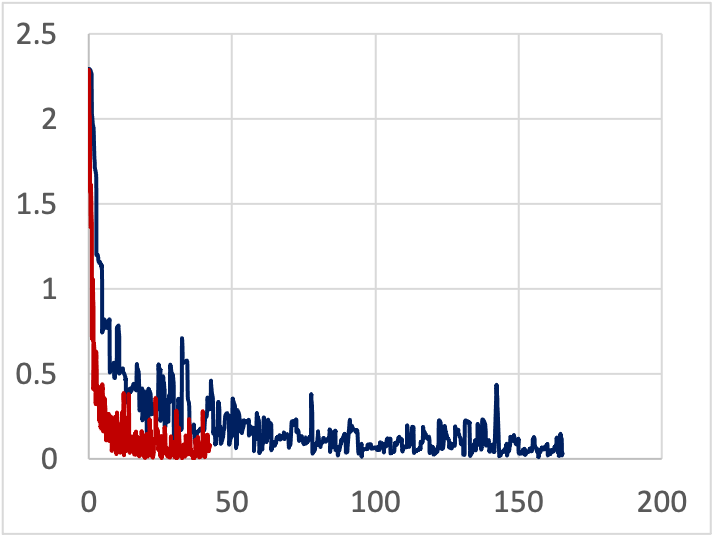
\includegraphics[width=\textwidth]{tape-lstm}
    \caption{LSTM-MNIST}
  \end{subfigure}
  ~ 
  \begin{subfigure}[t]{.24\textwidth}
    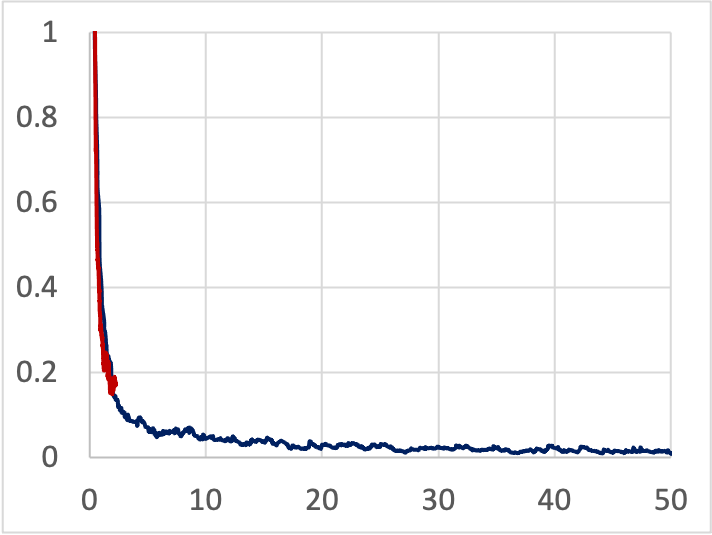
\includegraphics[width=\textwidth]{tape-simple2}
    \caption{SimpleCNN-GradientTape-2}
  \end{subfigure}
  ~
  \begin{subfigure}[t]{.24\textwidth}
    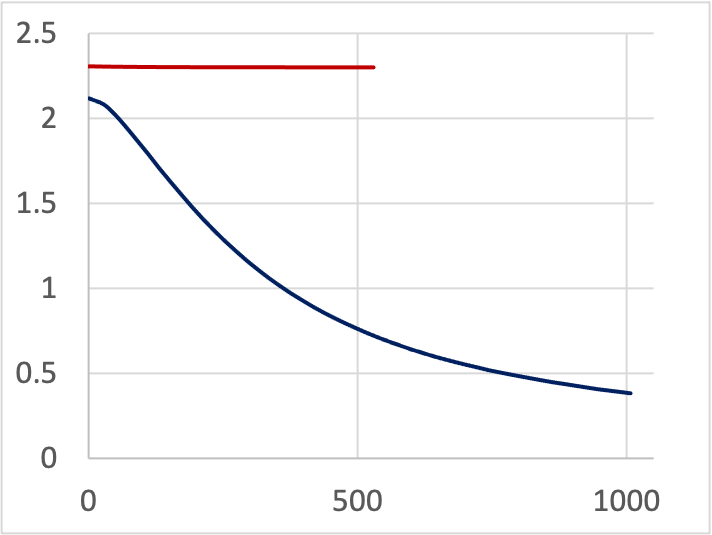
\includegraphics[width=\textwidth]{keras-cifar}
    \caption{VGG-CIFAR10}
  \end{subfigure}
  \par\bigskip
  \begin{subfigure}[t]{.24\textwidth}
    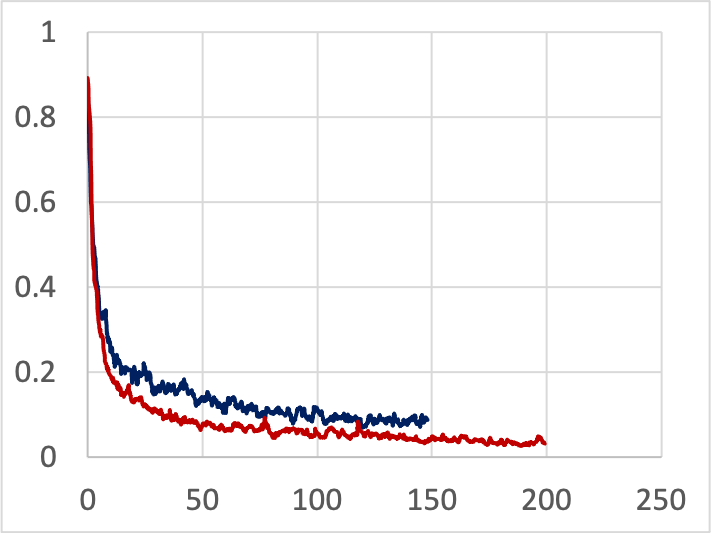
\includegraphics[width=\textwidth]{tf2-03}
    \caption{Play-with-MNIST}
  \end{subfigure}
  ~
  \begin{subfigure}[t]{.24\textwidth}
    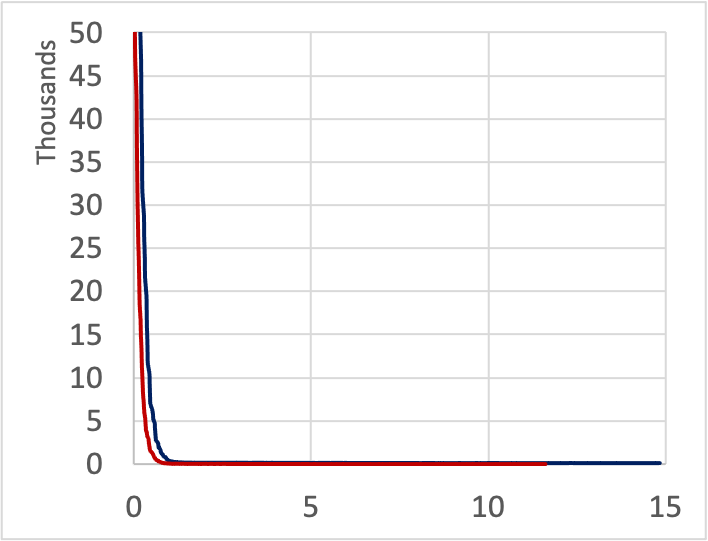
\includegraphics[width=\textwidth]{tf2-04}
    \caption{Linear-Regression}
  \end{subfigure} 
  ~ 
  \begin{subfigure}[t]{.24\textwidth}
    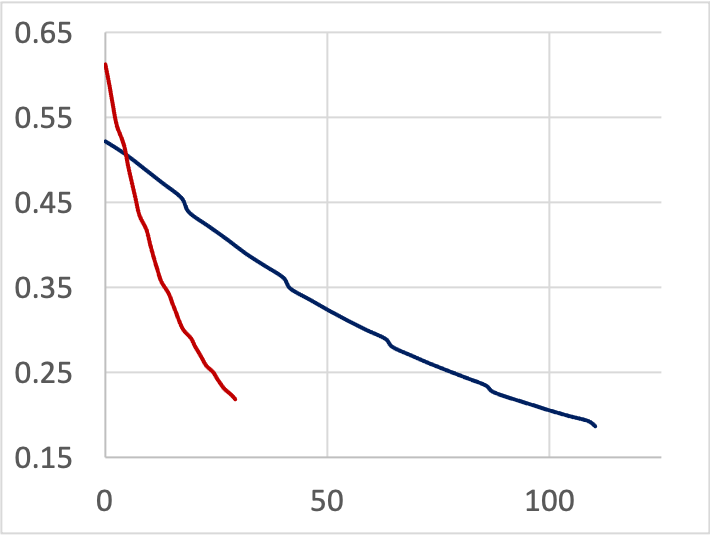
\includegraphics[width=\textwidth]{tf2-05}
    \caption{Fashion-MNIST}
  \end{subfigure}
  ~
  \begin{subfigure}[t]{.24\textwidth}
    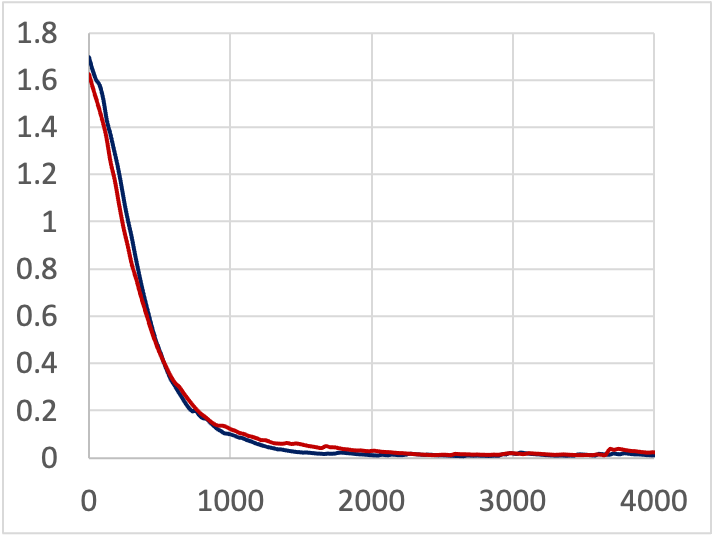
\includegraphics[width=\textwidth]{tf2-06}
    \caption{CIFAR10-VGG16}
  \end{subfigure}
  \par\bigskip
  \begin{subfigure}[t]{.24\textwidth}
    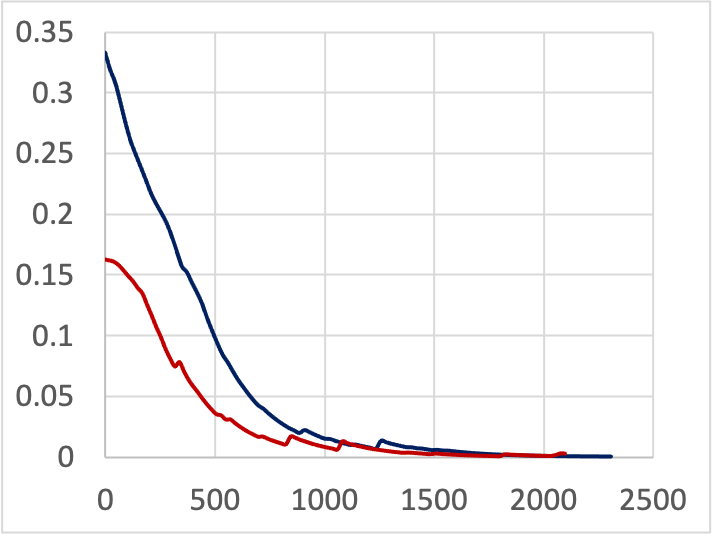
\includegraphics[width=\textwidth]{tf2-07}
    \caption{Inception-network}
  \end{subfigure}
  ~
  \begin{subfigure}[t]{.24\textwidth}
    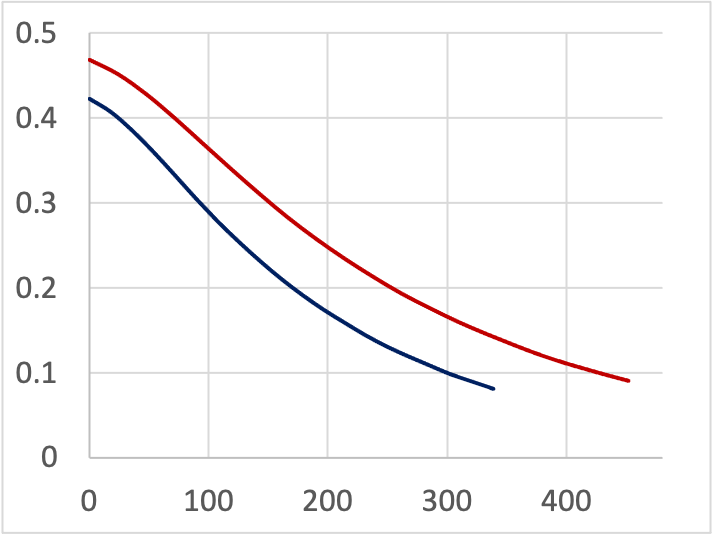
\includegraphics[width=\textwidth]{tf2-09}
    \caption{RNN-Sentiment-Analysis}
  \end{subfigure} 
  ~ 
  \begin{subfigure}[t]{.24\textwidth}
    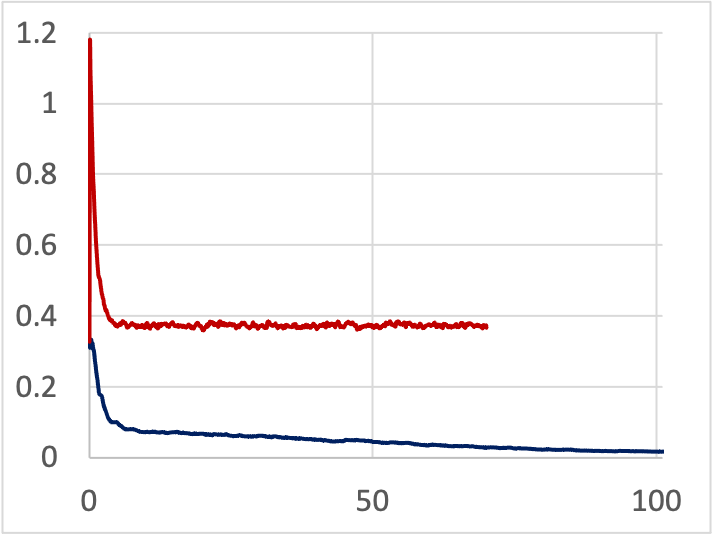
\includegraphics[width=\textwidth]{tf2-10}
    \caption{Stacked-LSTM-ColorBot}
  \end{subfigure}
  ~
  \begin{subfigure}[t]{.24\textwidth}
    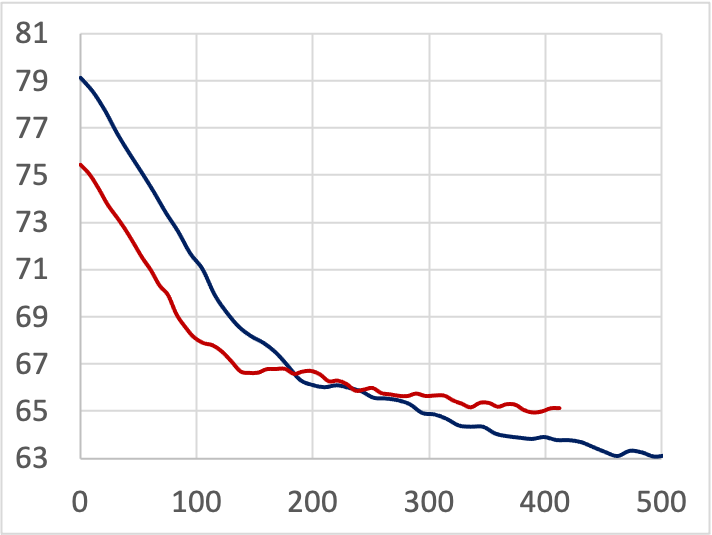
\includegraphics[width=\textwidth]{tf2-11}
    \caption{Auto-Encoder}
  \end{subfigure}
  \par\bigskip
  \begin{subfigure}[t]{.24\textwidth}
    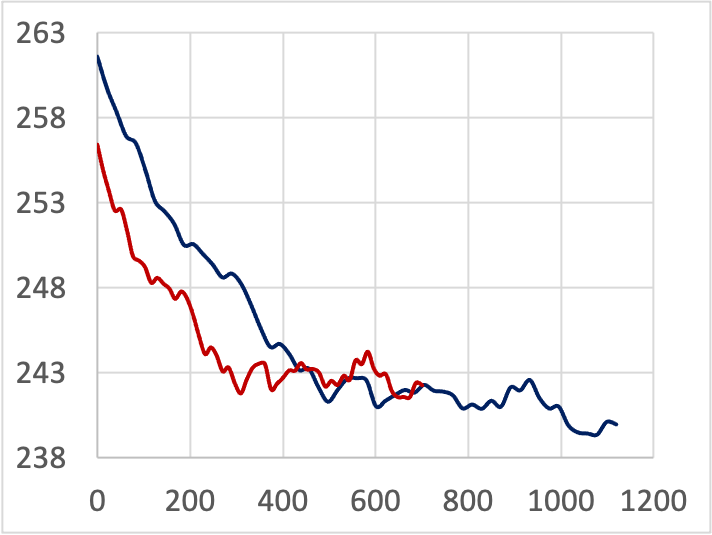
\includegraphics[width=\textwidth]{tf2-12}
    \caption{Variational-Auto-Encoder}
  \end{subfigure}
  ~
  \begin{subfigure}[t]{.24\textwidth}
    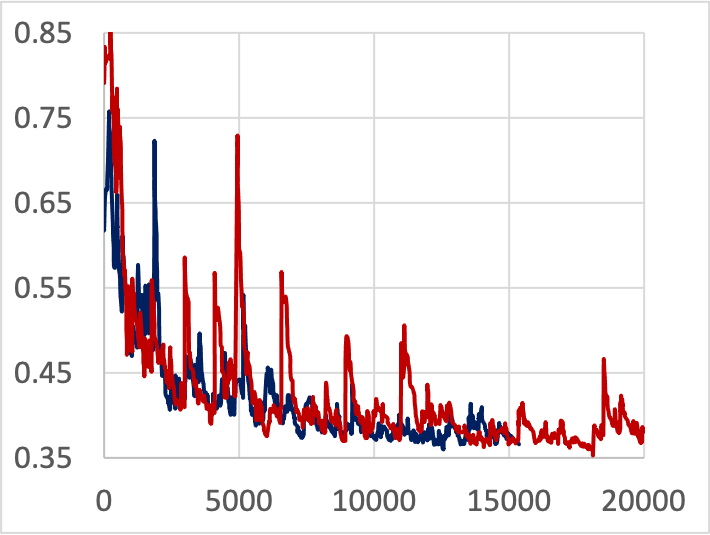
\includegraphics[width=\textwidth]{tf2-13}
    \caption{DCGAN}
  \end{subfigure} 

  \caption{Distributed training experiment result time-loss graphs.}
  \begin{tabular}{r@{: }l r@{: }l}
    X-axis & Time (seconds) & Y-axis & Loss value\\
    Blue line & ORG loss, smoothed & Red line & HVD loss, smoothed\\ 
  \end{tabular}
  \label{fig:eval:train}
\end{figure}

The results of the distributed traininig experiment 
are shown in the figure \ref{fig:eval:train}.
The lines represent the smoothed loss values;
blue lines correspond to the \textbf{ORG} model training
and the red lines correspond to the \textbf{HVD} model training.
As shown in the figure, all of the training data show that
the loss value decreases over time, meaning that the training
process is valid.

The distributed training experiment result show that the 8 out of 17 transformed
models show speedup in distributed traininig. The result is rather surprising,
considering that the distributed training itself is successfully executed
without errors. To further investigate the factors that influence the
training speed in the distributed training, 
we performed additional distributed training of some models with
different hyperparameters.

\begin{figure}[!ht]
  \centering
  \begin{subfigure}[t]{.24\textwidth}
    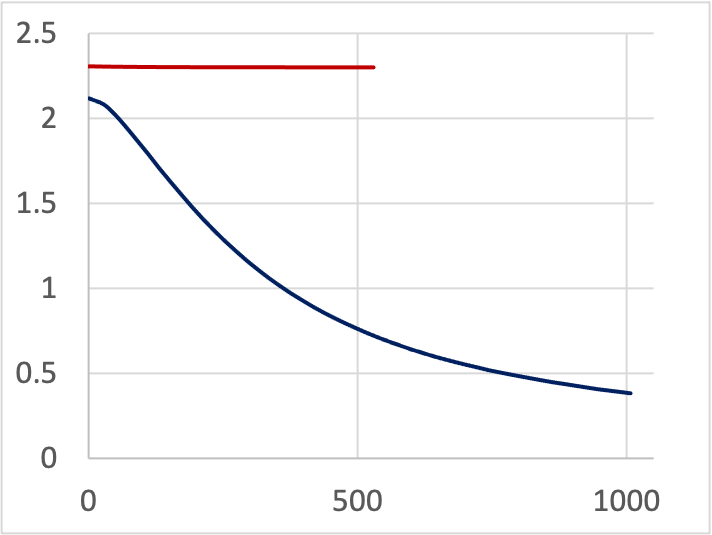
\includegraphics[width=\textwidth]{keras-cifar}
    \caption{VGG-CIFAR10 model with lr=0.001 (default value)}
  \end{subfigure}
  ~
  \begin{subfigure}[t]{.24\textwidth}
    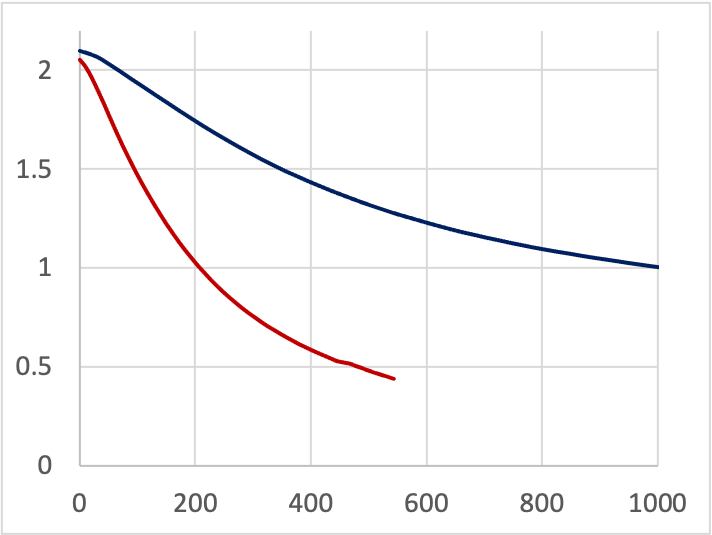
\includegraphics[width=\textwidth]{cifar-1e4}
    \caption{VGG-CIFAR10 model with lr=0.0001}
  \end{subfigure} 
  ~ 
  \begin{subfigure}[t]{.24\textwidth}
    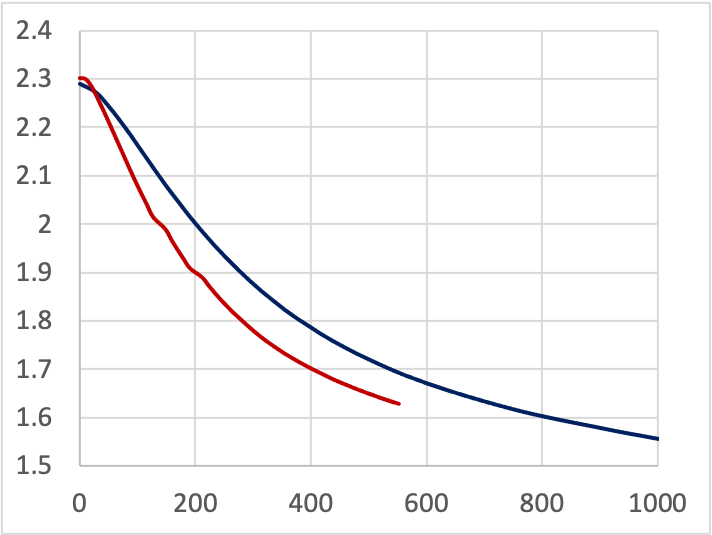
\includegraphics[width=\textwidth]{cifar-1e5}
    \caption{VGG-CIFAR10 model with lr=0.00001}
  \end{subfigure}
  ~
  \begin{subfigure}[t]{.24\textwidth}
    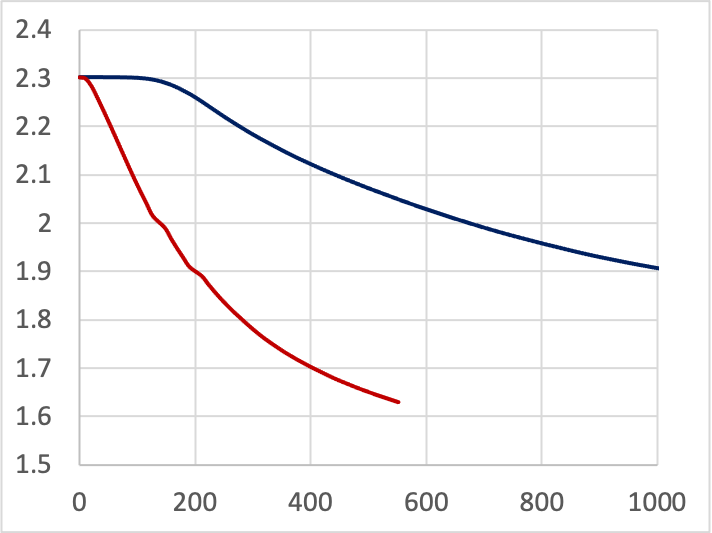
\includegraphics[width=\textwidth]{cifar-1e6}
    \caption{VGG-CIFAR10 model with lr=0.000001}
  \end{subfigure}

  \caption{Distributed training experiments of VGG-CIFAR10 model with different learning rates.}
  \begin{tabular}{r@{: }l r@{: }l}
    X-axis & Time (seconds) & Y-axis & Loss value\\
    Blue line & ORG loss, smoothed & Red line & HVD loss, smoothed\\ 
  \end{tabular}
\end{figure}


The results show that the training speed difference between single-GPU and
distributed training can differ according to the model hyperparameters
such as the learning rate. The fact that various combinations of hyperparameters
must be considered and experiement to reach optimal training speed is 
well-known in ML community. This problem also applies to distributed training,
where optimial hyperparameters should be re-searched after the training
code is transformed. Our transformation tool do not target to search the 
optimal hyperparameters, although we do implement the guidelines from the
official Horovod documents to scale learning rate and epoch numbers
by number of the GPUs.  

Although the automatically transformed model codes may need additional
tuning, our transformation tool effectively reduces
burdens of manually rewriting the training codes.
By applying our tool, the users can quickly change the single-GPU-based
models into the distributed model and initiate the tranining.
During the training process, the user may monitor training-related measurements
such as per-epoch loss and decide to tune the hyperparameters.
From the transformed training code, the user is able to quickly locate the
hyperparameter variables, which suffer none-or-minimal changes of their locations
from the original code.
Therefore, the users of our tool can quickly iterate the process of
training, evaluating and tuning without rewriting the
training code with manual investigation on the library documentations and
the model code.
